\documentclass[xcolor=dvipsnames]{beamer}
\usepackage[utf8]{inputenc}
\usepackage[T1]{fontenc}

\usetheme{AnnArbor}
\usepackage{dsfont}
\usepackage{amsmath}
\usepackage{caption}
\usepackage{hyperref}
\usepackage{xcolor}
\usepackage{color}
\usepackage{commath}
\usepackage{physics}
\usepackage{enumerate}
\usepackage{hyperref}

%\usepackage[backend=bibtex, style=authoryear-comp]{biblatex}

\setbeamertemplate{bibliography item}{\insertbiblabel}
\beamertemplatenavigationsymbolsempty

\usepackage{filecontents}
\begin{filecontents}{\jobname.bib}
@article{blei2003latent,
  title={Latent dirichlet allocation},
  author={Blei, David M and Ng, Andrew Y and Jordan, Michael I},
  journal={Journal of machine Learning research},
  volume={3},
  number={Jan},
  pages={993--1022},
  year={2003}
}
@article{roberts2016model,
  title={A model of text for experimentation in the social sciences},
  author={Margaret E. Roberts and Brandon M. Stewart and Edoardo M. Airoldi},
  journal={Journal of the American Statistical Association},
  volume={111},
  number={515},
  pages={988--1003},
  year={2016},
  publisher={Taylor \& Francis}
}
\end{filecontents}
\usepackage[style=authoryear]{biblatex}
\renewcommand*{\nameyeardelim}{\addcomma\addspace}
\addbibresource{\jobname.bib}

\newcommand{\customcite}[1]{\citeauthor{#1} (\citeyear{#1})}

\newtheorem{satz}{Satz}

\setbeamertemplate{footline}[page number]

\usecolortheme{seagull}
\setbeamercolor{frametitle}{fg=blue,bg=White}

%\DeclareMathOperator*{\argmax}{arg\, max}
%\DeclareMathOperator*{\argmin}{arg\, min}
%\setbeamertemplate{section in toc}[sections numbered]
%\setbeamertemplate{subsection in toc}[subsections numbered]
%\AtBeginSection[]
%{
%\begin{frame}
%\frametitle{Überblick}
%\tableofcontents[currentsection]
%\end{frame}
%}
%
%\AtBeginSubsection[
% {\frame<beamer>{\frametitle{Überblick}   
%  \tableofcontents[currentsection,currentsubsection]}}%
%]%
%{
 % \frame<beamer>{ 
 %   \frametitle{Überblick}   
   % \tableofcontents[currentsection,currentsubsection]}
%}

\title{Twitter in the Parliament - A Text-based Analysis of German Political Entities}
%\author{Patrick Schulze}
\date{7. Juli 2020}
\author[author1]{Patrick Schulze, Simon Wiegrebe\\[10mm]{\small Supervisors:\\ Prof. Dr. Christian Heumann, Prof. Dr. Paul W. Thurner}}

\begin{document}

\begin{frame}
\titlepage
\end{frame}

%\begin{frame}
%\frametitle{Überblick}
%\tableofcontents[]
%\end{frame}

\section{}
\begin{frame}
\frametitle{Outline}
\begin{itemize}
\item Introduction
\item Topic Modeling: Motivation and Theory
\item Data: Collection and Preprocessing
\item Model Selection and Global Characteristics
\item Metadata Analysis
\item Causal Inference
\item Discussion
\end{itemize}
\end{frame}

\begin{frame}
\frametitle{Introduction}
\begin{itemize}
\item Rise in popularity of social media is producing huge amounts of data, especially text.
\item \textit{Politics} is a field of particular interest in the context of social media and big data (Brexit, 2016 presidential election in the US, Facebook data scandal).
\item Simultaneously, advances in \textit{Natural Language Processing} (NLP) are providing tools of analysis for such data.
\item One instance of such analysis is the discovery and exploration of latent thematic clusters within text - \textit{topic analysis}.
\item In this project, we apply the \textit{Structural Topic Model} (STM) to a self-created dataset containing Twitter posts by members of the German Bundestag (and a variety of metadata) 
\end{itemize}
\end{frame}

\begin{frame}
\frametitle{Topic Modeling: Motivation and Theory}
\framesubtitle{Notation and Terminology}
\begin{itemize}
\item A \textit{word} is an instance of a vocabulary of $V$ unique \textit{terms}.
\item A \textit{document} $d \in \{1,\dots,D\}$ is a sequence of words of length $N_{d}$. The $n$-th word of document $d$ is denoted by $w_{d,n}$.
\item A \textit{corpus} is a collection (or set) of $D$ documents. Therefore, $d \in \{1,\dots,D\}$ means that our corpus contains $D$ documents.
\item A \textit{topic} $k \in \{1,\dots,K\}$ is a latent thematic cluster within a text corpus. That is, we imply a corpus can be represented by $K$ topics.
\item A \textit{topic-word distribution} $\boldsymbol{\beta}$ is a probability distribution over words. We denote the word distribution corresponding to the $k$-th topic by $\boldsymbol{\beta}_k$.
\item A \textit{topic assignment} $\boldsymbol{z}_{d,n}$ assign $w_{d,n}$ to a specific topic $k \in \{1,\dots,K\}$. We represent the word distribution for $w_{d,n}$ as $\boldsymbol{\beta}_{d,n}$.
\item \textit{Topic proportions} $\boldsymbol{\theta}_d$ are the proportions of the document $d$'s terms assigned to each of the topics. $\sum_{k=1}^{K}\theta_{d,k}=1$, for all $d \in \{1,\dots,D\}$.
\end{itemize}
\end{frame}

\begin{frame}
\frametitle{Topic Modeling: Motivation and Theory}
\framesubtitle{\textit{Latent Dirichlet Allocation} (LDA)}
\begin{itemize}
\item LDA by \textcite{blei2003latent} is the first probabilistic topic model.
\item Its generative process for each document $d \in \{1,\dots,D\}$ is:
\item[] 
	\begin{enumerate}[{1)}]
	\item Draw topic proportions $\boldsymbol{\theta}_d \sim \text{Dir}_K(\boldsymbol{\alpha})$.
	\item For each word $n \in \{1,\dots,N_d\}$:
		\begin{enumerate}[{a)}]
		\item Draw a topic assignment $\boldsymbol{z_{d,n}} \sim \text{Multinomial}_K(\boldsymbol{\theta}_d)$.
		\item Draw a word $w_{d,n} \sim \text{Multinomial}_V(\boldsymbol{\beta}_{d,n})$.
	\end{enumerate}
\end{enumerate}
\item Graphical model representation (\textcite{roberts2016model}, p.\ 990): 
	\begin{figure}[h!]
  	\centering
  	%\captionsetup{justification=centering,margin=2cm}
  	\hspace*{-1cm}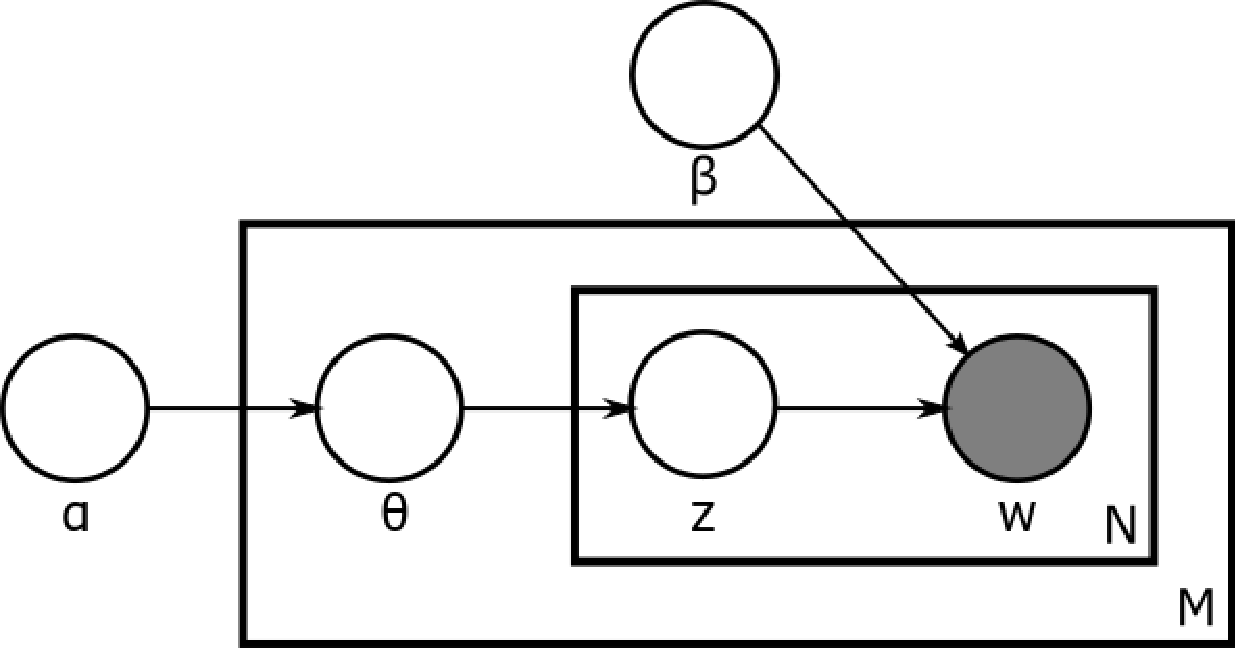
\includegraphics[scale = 0.3]{../plots/presentation/lda_graphical.pdf}
  	%\caption{Graphical model representation of the STM (from \textcite{roberts2016model}, p.\ 990).}
	\end{figure}
\end{itemize}
\end{frame}

\begin{frame}
\frametitle{Topic Modeling: Motivation and Theory}
\framesubtitle{\textit{Latent Dirichlet Allocation} (LDA)}
\begin{itemize}
\vspace{-0.5cm}
\item The topic assignment of a document's words can be illustrated as follows:
	\vspace{-0.5cm}
	\begin{figure}[h!]
  	\centering
  	%\captionsetup{justification=centering,margin=2cm}
  	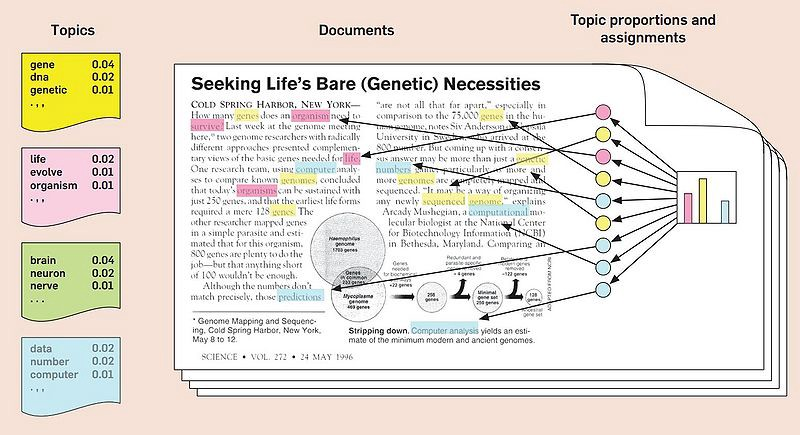
\includegraphics[scale = 0.4]{../plots/presentation/lda_topic_assignment.jpeg}
  	%\caption{Graphical model representation of the STM (from \textcite{roberts2016model}, p.\ 990).}
	\end{figure}

\end{itemize}
\end{frame}

\begin{frame}
\frametitle{Data}
\framesubtitle{Data Collection}
\begin{itemize}
\item MP-level data was scraped from \url{www.bundestag.de/abgeordnete} using Python's \textit{BeautifulSoup} and a \textit{selenium web driver}
\item[] 
	\begin{figure}[h!]
  	\centering
  	%\captionsetup{justification=centering,margin=2cm}
  	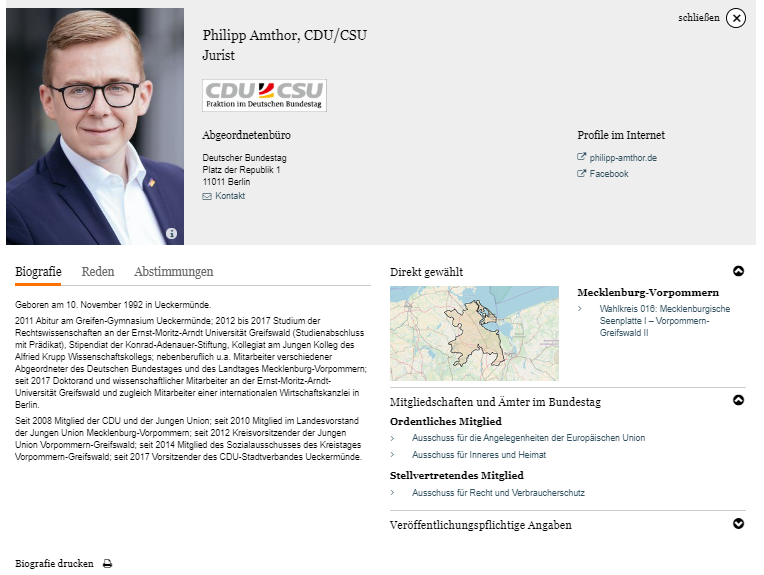
\includegraphics[scale = 0.42]{../plots/presentation/amthor.png}
  	%\caption{Graphical model representation of the STM (from \textcite{roberts2016model}, p.\ 990).}
	\end{figure}
\item Socioeconomic data and 2017 German federal election results were extracted from \url{www.bundeswahlleiter.de}.
\end{itemize}
\end{frame}

\begin{frame}
\frametitle{Data}
\framesubtitle{Data Collection}
\begin{itemize}
\item Tweets (and further Twitter features) were downloaded via the official Twitter API using Python's \textit{tweepy} library.
\item Monthly tweets (after dropping MPs without electoral district) for our period of analysis, September 24, 2017 through April 24, 2020:
	\begin{figure}[h!]
  	\centering
  	%\captionsetup{justification=centering,margin=2cm}
  	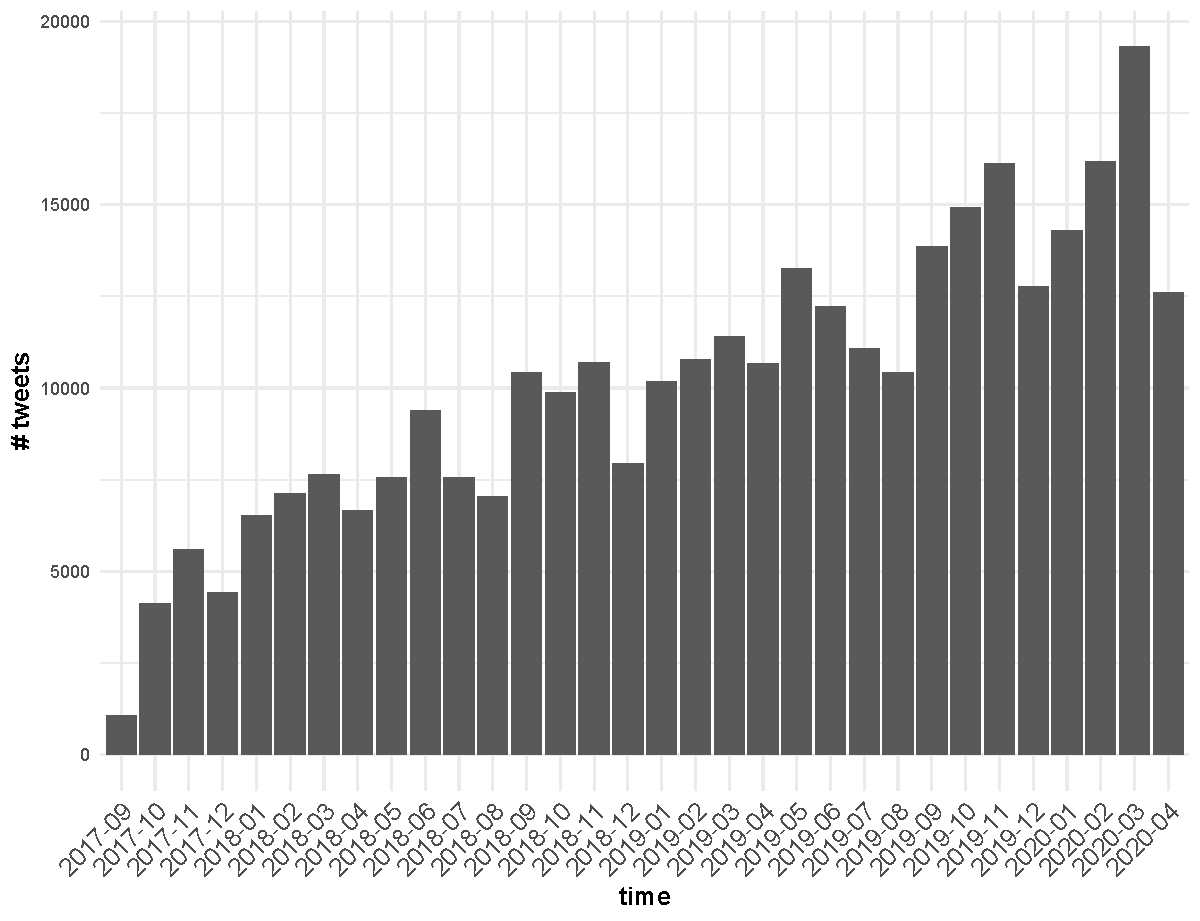
\includegraphics[scale = 0.30]{../plots/3/monthly_tweets.pdf}
  	%\caption{Graphical model representation of the STM (from \textcite{roberts2016model}, p.\ 990).}
	\end{figure}
\item Henceforth, we grouped each MP's tweets on a monthly basis.
\end{itemize}
\end{frame}

\begin{frame}
\frametitle{Data}
\framesubtitle{Data Preprocessing}
\begin{itemize}
\item For preprocessing, we used the \textit{quanteda} package in R.
\item We immediately transcribed German umlauts (\"a, \"o, \"u) and ligature (\ss) and removed hyphens due to the presence of compound words in the German language (e.g., \textit{Corona-Krise} vs \textit{Coronakrise}).
\item Next, we transformed the text data into a document-feature matrix (DFM), converted all characters to lowercase, and removed stopwords, units, interjections, etc.
\item Finally, we performed word stemming, which cuts off word endings to remove discrepancies arising purely from declensions or conjugations
(e.g., \textit{politisch} $\rightarrow$ \textit{polit}).
\end{itemize}
\end{frame}

\begin{frame}
\frametitle{Model Selection and Global Characteristics}
\framesubtitle{Model Selection}
\begin{itemize}
\item XXX
\item XXX
\end{frame}

\begin{frame}
\frametitle{Bibliography}
\printbibliography
\end{frame}
\end{document}